%%%%%%%%%%%%%%%%%%%%%%%%%%%%%%%%%%%%%%%%%%%%%%%%%%%%%%%%%%%%%%%%%%%%%%%%%%%%%%
%%%%%%%%%%%%%%%%%%%%%%%%%%%%%%%%%%%%%%%%%%%%%%%%%%%%%%%%%%%%%%%%%%%%%%%%%%%%%%
%%
%% Dokumentacia k semestralnemu projektu z PRL2
%%
%%%%%%%%%%%%%%%%%%%%%%%%%%%%%%%%%%%%%%%%%%%%%%%%%%%%%%%%%%%%%%%%%%%%%%%%%%%%%%
%%%%%%%%%%%%%%%%%%%%%%%%%%%%%%%%%%%%%%%%%%%%%%%%%%%%%%%%%%%%%%%%%%%%%%%%%%%%%%
\documentclass[11pt,a4paper,titlepage,final]{article}

% cestina a fonty
\usepackage[czech]{babel}
\usepackage[T1]{fontenc}
\usepackage[utf8]{inputenc}
% balicky pro odkazy
\usepackage[bookmarksopen,colorlinks,plainpages=false,urlcolor=blue,unicode]{hyperref}
\usepackage{url}
% obrazky
\usepackage[dvipdf]{graphicx}
% velikost stranky
\usepackage[top=3.5cm, left=2.5cm, text={17cm, 24cm}, ignorefoot]{geometry}
\usepackage{fancyhdr}

\begin{document}
\raggedright\large{\textbf{Projekt z predmetu PRL Martin Maga (xmagam00) \\Carry Look Ahead Parallel Binary Adder}}

\section{Teoretické rozobratie algoritmu}
Algoritmus je postavený na myšlienke sčítania 2 binárnych čísel pomocou binárnych sčítačiek (reprezentovanými procesormi), ktoré na vstupe majú i-tý bit zo vstupných binárnych čísel a prenos. od predchádzajúcej sčítačky (procesoru). Jednotlivé sčítačky generajú pri sčitaní i-tého bitu prenos $c_i$, ktorý sa prenáša do ďalšej sčítačky, tj. pri sčítaní i-tého bitu sa generuje prenos $c_i$, ktorý sa použije v nasledujúcom výpočte pri výpočte i+1-teho bitu, pri ktorom sa generuje $c_{i+1}$. Pri tomto algoritme je potreba ešte pred samostatným výpočtom vyriešiť všetky bity prenosu $c_{n-1}$ \ldots $c_0$, tzv pole D, ktoré obsahuje všetky prenosy aby sme mohli priamo paralelne spočítať $z_i$ = $x_i$ + $y_i$ + $c_i$. Pri výpočte tohto pola prenosov používame algoritmus scan.

\section{Časová zložitosť}
Časová zložitosť tohto algoritmu je priamo ovplyvnená tým, že pred zahájením samostného sčítania dvoch binárnych čísel je nutné predvypočítať všetky bity prenosu $c_{n-1}$ \ldots $c_0$. Všetky bitu prenosu dostanme presne po log n krokoch prostredníctvom algoritmu scan. Samostný výpočet následne zabere presne 1 krok pre n bitové číslo, teda pre n procesorov. Časová zložitosť algoritmu scan je priamo ovplyvnená použitou výpočtovov, ktorá je binárny vyvážený strom. Sumy hodnôt sa postupne predávajú od listov až po koreň. Výsledná hodnota sa dostane do koreňa presne po log n krokoch. Celková časová zložitosť tohto algoritmu je: \textbf{t(n) = log n + 1}.

\section{Priestorová zložitosť}
V tomto algoritme používame binárne sčítačky, keďže celý výpočet je paralelizovaný každú binárnu sčítačku reprezentuje 1 procesor. Celkovo pre n-bitové číslo potrebuje n procesorov, pričom každú má na vstupe práve 1 bit (i-tý bit) z každého vstupného čisla a prenos z predchádzajúceho výpočtu z binárnej sčítačky, ktorý sme si ale predvypočítali algoritmom scan.Priestorová zložitosť je: \textbf{p(n) = n}


\section{Celková cena algoritmu}
Celková cena algoritmu je: c(n) = p(n) * t(n). Pre náš algoritmus dostávame hodnotu: c(n) = (log n + 1)*n = $n * log n$ (pri zanedbaní nejakých premenných). Celková cena riešenia je semilogaritická, je ešte optimálne pre paralelné riešenie.

\section{Implementácia}
Pri implementácií algoritmu Carry Look Ahead Parallel Binary Adder bola použivá knižnica OpenMPI spolu s jazykom C+. Táto knižnica umožňuje implementáciu algoritmov paralelne, pričom vytvára procesory (similuje ich), ktoré komunikujú prostredníctvom správ. Program clapba.cpp po preložení paralelne v prvom ktorku vypočíta algoritmom scan sumu prefixov. Jednotlivé čísla pre výpočet načíta zo súboru "numbers", ktorý obsahuje 2 čísla oddelené znakom nového riadku ("\\n"). V ďalšom kroku overí, či majú rovnakú dĺžku v opačnom prípade doplní pred číslo s menším počtom bitov 0.

Po vypočítaní jednotlivých hodnôt prepošle "prvý procesr" (tj procesor s hodnotou $my_id$ 0) i-tý bit prenosu i-tému procesoru spolu s i-tým bitom 1. a 2. čísla. I-tý procesor po obdržaní prenosu a bitov z oboch čísel zaháji výpočet.
Sčíta tieto 2 bity spolu so sumou podľa vzorca: $z_i$ = $x_i$ + $y_i$ + $c_i$. Pokiaľ výpočet $z_i$ pretečie indikuje procesor pretečenie hláškou "overflow" na štandarný výstup spolu s číslom procesoru a následne sa procesor ukončí.

Celý algoritmu skončí v prípade, že skončí posledný procesor. Treba podotknúť,že indexy procesoru dodržujú štruktúru 2*n-2, tj procesor spracuvávajúci n-tý bit má index 2*n-2.

\section{Komunikačný protokol}
Na nasledujúcom obrázku je zobrazený komunikačný protokol:
 \begin{figure}[h]

\begin{center}
\scalebox{0.15}{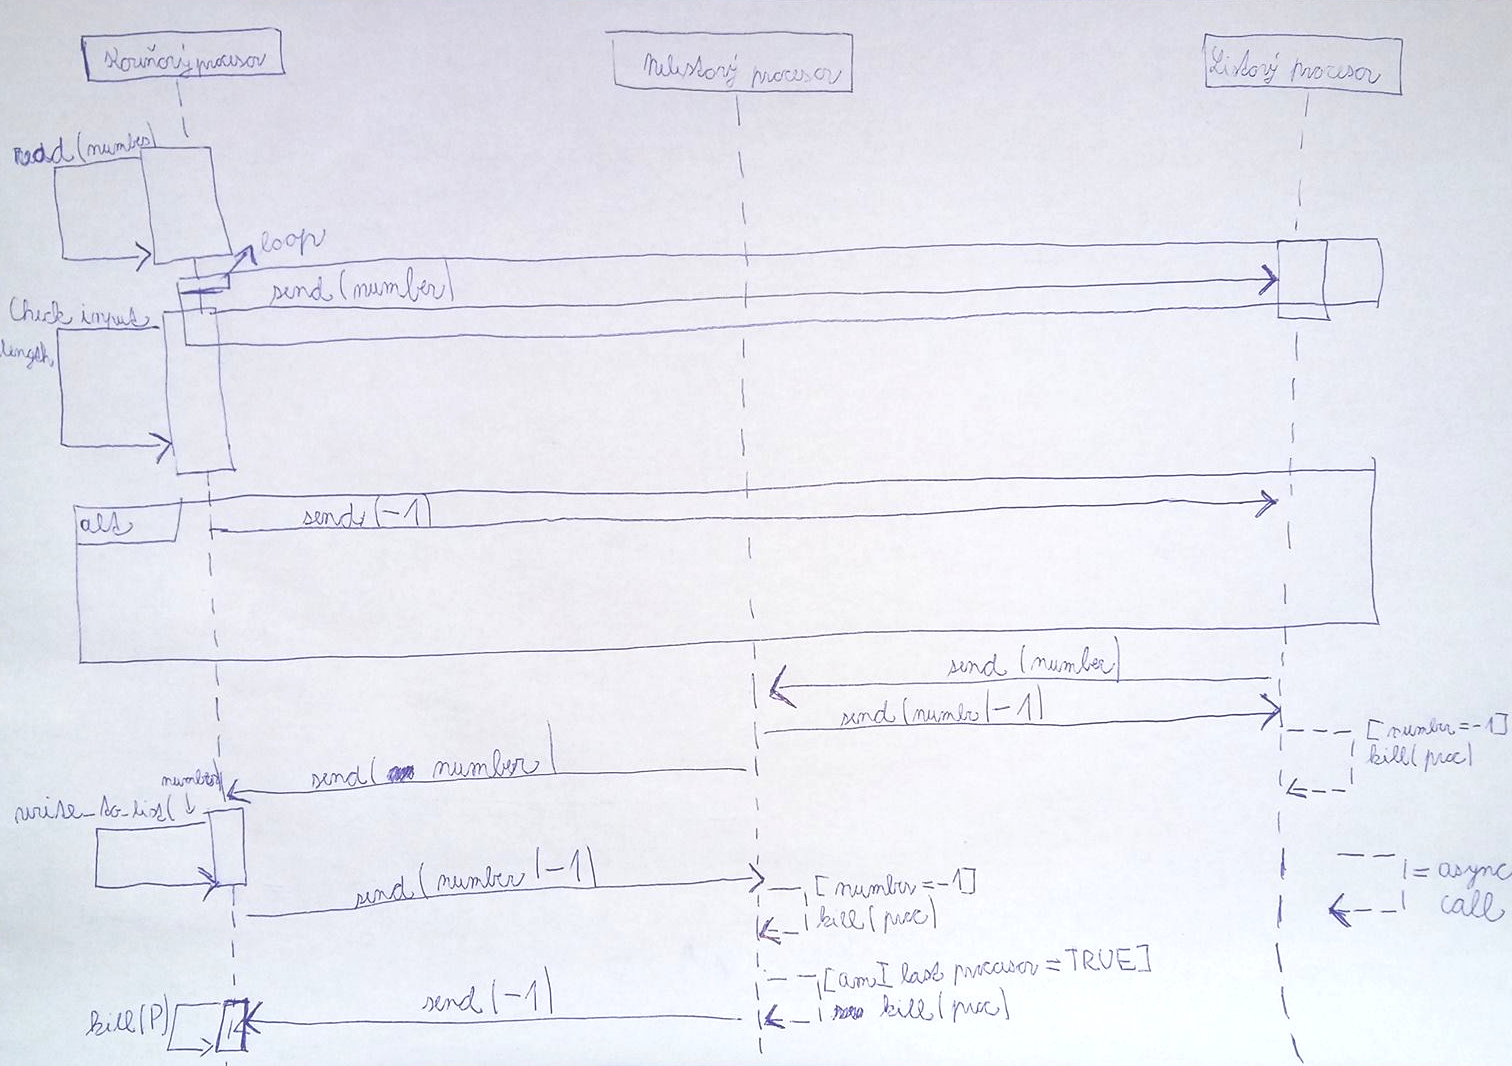
\includegraphics{img/diagram.eps}}
\caption{Sekvenčí diagram popísujúci komunikáciu}
\end{center}

\end{figure}


\section{Experimenty}
V tejto kapitole sme overovali časovú zložitosť, ktorá je približne logaritmická. Z tohto môžme predpokladať, že výsledný graf bude mať tvar logaritmickej krivky. Pre overenie sme vykonali experiment nasledovne: Ako vstup sme postupne spúštali skript test.sh nasledovne: 1.beh test.sh 1, 2. beh test.sh 2 ,3.beh test.sh 3, 4.beh test.sh 4, 5.beh test.sh 5, 6.beh test.sh 6, 7.beh test.sh 7, 8.beh test.sh 8, 9.beh test.sh 9, 10.beh test.sh 10, 11.beh test.sh 11, 12.beh test.sh 12, 13.beh test.sh 13, 14.beh test.sh 14, 15.beh test.sh 15, 16.beh test.sh 16, 17.beh test.sh 17, 18.beh test.sh 18, 19.beh test.sh 19, 20.beh test.sh 20.

Algoritmus sme spúštali na serveri merlin(Linux merlin.fit.vutbr.cz 3.12.56 $x86\_64$ GNU/Linux). Pre správnosť výsledkov sme každú konfiguráciu spustili 100x a výsledný čas som spriemeroval. Treba spomenúť, že nebolo možné overiť riešenie pre väčší počet hodnôt, keďže server merlin nedovoluje spustiť program s väčším počtu procesorov.

Z implementačného hľadiska treba podotknúť, že meranie je realizované funkcou $"MPI_Wtime()"$, ktorá vracia počet sekúnd. Tento funkcia sa volá na začiatku a na konci pre koreňový procesor.
 \begin{figure}[h]

\begin{center}
\scalebox{0.5}{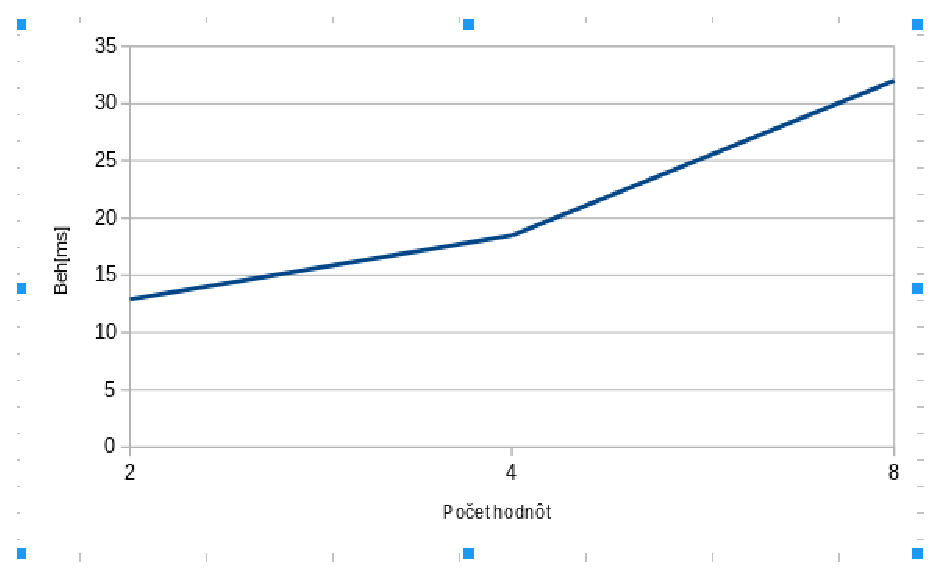
\includegraphics{img/mes.eps}}
\caption{Graf časovej závislosti počtu vstupných hodnôt a behu programu v ms}
\end{center}

\end{figure}

\section{Záver}
Implementovali sme algoritmus Carry Look Ahead Parallel Binary Adder s knižnicou OpenMPI. Rovnako sme odvodili teoretickú časovú, priestorovú a celkovú zložitosť algoritmu, ktorú sme experimentom aj potvrdili.
\end{document}



